\documentclass[tikz,border=8pt]{standalone}
\usepackage{pgfplots}
\pgfplotsset{compat=1.18}
\begin{document}
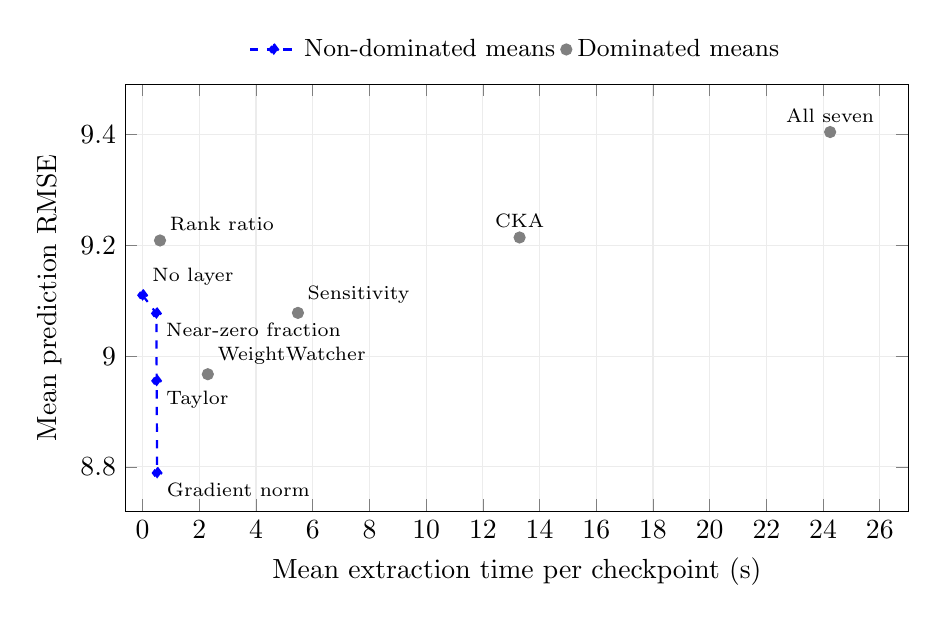
\begin{tikzpicture}
\begin{axis}[
    width=0.95\linewidth,
    height=7cm,
    xmin=-0.6, xmax=27,
    ymin=8.72, ymax=9.49,
    xlabel={Mean extraction time per checkpoint (s)},
    ylabel={Mean prediction RMSE},
    grid=major,
    grid style={gray!15},
    clip=false,
    legend style={
        at={(0.5,1.03)},
        anchor=south,
        legend columns=2,
        draw=none,
        font=\small
    }
]
\addplot[
    blue, dashed, thick, mark=diamond*
] coordinates {
    (0.0000,9.1098)
    (0.4869,9.0770)
    (0.4942,8.9553)
    (0.5108,8.7890)
};
\addlegendentry{Non-dominated means}

\addplot[
    only marks, gray, mark=*
] coordinates {
    (2.2988,8.9673)
    (0.6130,9.2087)
    (5.4777,9.0780)
    (13.2964,9.2141)
    (24.2493,9.4044)
};
\addlegendentry{Dominated means}

\node[anchor=south west,font=\scriptsize]
    at (axis cs:0.0000,9.1098) {No layer};
\node[anchor=north west,font=\scriptsize]
    at (axis cs:0.4869,9.0770) {Near-zero fraction};
\node[anchor=north west,font=\scriptsize]
    at (axis cs:0.4942,8.9553) {Taylor};
\node[anchor=north west,font=\scriptsize]
    at (axis cs:0.5108,8.7890) {Gradient norm};
\node[anchor=south west,font=\scriptsize]
    at (axis cs:2.2988,8.9673) {WeightWatcher};
\node[anchor=south west,font=\scriptsize]
    at (axis cs:0.6130,9.2087) {Rank ratio};
\node[anchor=south west,font=\scriptsize]
    at (axis cs:5.4777,9.0780) {Sensitivity};
\node[anchor=south,font=\scriptsize]
    at (axis cs:13.2964,9.2141) {CKA};
\node[anchor=south,font=\scriptsize]
    at (axis cs:24.2493,9.4044) {All seven};
\end{axis}
\end{tikzpicture}
\end{document}
